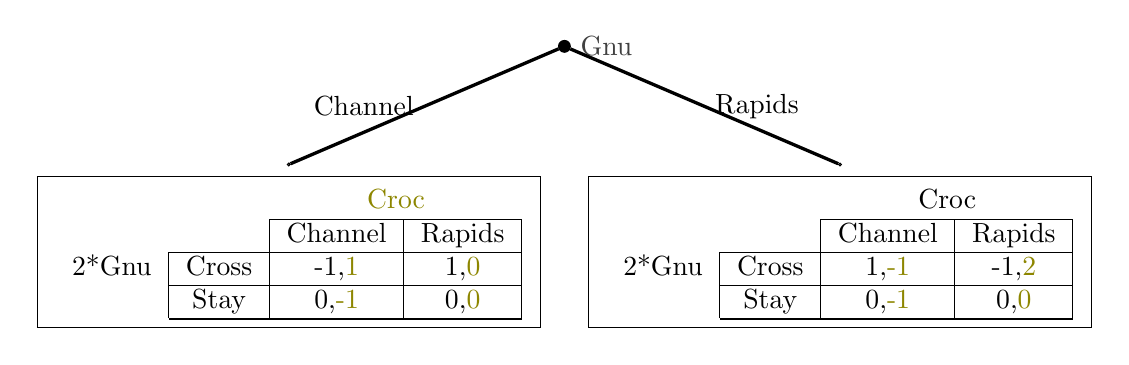
\begin{tikzpicture}[edge from parent/.style={draw, very thick}]
    \tikzstyle{solid node}=[circle,draw,inner sep=1.5,fill=black]
    \tikzstyle{hollow node}=[circle,draw,inner sep=.25]
    \tikzstyle{level 1}=[level distance=15mm,sibling distance=7cm]
    \tikzstyle{pruned edge from parent}=[draw, very thick, darkgray, dashed, -]
    
    \node(0)[solid node,label=right:{\color{darkgray} Gnu}]{}
      child{node[hollow node,label=below:{
        \fbox{
        \begin{tabular}{*{4}{c|}}
           \multicolumn{2}{c}{} & \multicolumn{2}{c}{\color{olive} Croc} \\\cline{3-4}
           \multicolumn{1}{c}{} &       & Channel & Rapids \\\cline{2-4}
           \multirow{2}*{Gnu}   & Cross & -1,{\color{olive}1}  & 1,{\color{olive}0}   \\\cline{2-4}
                                & Stay  & 0,{\color{olive}-1}  & 0,{\color{olive}0}   \\\cline{2-4}
        \end{tabular}
        }
      }]{}
          edge from parent node[left]{Channel}
      }
      child{node[hollow node,label=below:{
        \fbox{
        \begin{tabular}{*{4}{c|}}
           \multicolumn{2}{c}{} & \multicolumn{2}{c}{Croc} \\\cline{3-4}
           \multicolumn{1}{c}{} &       & Channel & Rapids \\\cline{2-4}
           \multirow{2}*{Gnu}   & Cross & 1,{\color{olive}-1}  & -1,{\color{olive}2}   \\\cline{2-4}
                                & Stay  & 0,{\color{olive}-1}  &  0,{\color{olive}0}   \\\cline{2-4}
        \end{tabular}
        }
      }]{}
          edge from parent node[right]{Rapids}
      }
      ;
\end{tikzpicture}
